\documentclass[11pt]{article}
% packages
\usepackage[utf8]{inputenc}
\usepackage[T1]{fontenc}
\usepackage{geometry}
\usepackage[pdftex]{graphicx}
\usepackage{graphicx}
\usepackage{tabularx}
\usepackage{dsfont}
\usepackage{multirow}
\usepackage{amsmath,amsfonts,amssymb}
\usepackage{subcaption}
\usepackage{authblk}
\usepackage{placeins}
%hyperlinks options
\usepackage{hyperref}
\hypersetup{colorlinks=true,linkcolor=blue,filecolor=magenta,urlcolor=cyan,citecolor=cyan}
%bib options
\usepackage[backend=biber,style=authoryear,bibstyle=authoryear,natbib=true,
giveninits=true,uniquename=false,uniquelist=false,% firstinits=false,
maxcitenames=2,date=year, maxbibnames=99,url=false]{biblatex}
\geometry{left=20mm, top=20mm, right=20mm}
%float barrier
\usepackage{placeins}
 \addbibresource{Thèse.bib}
\title{Chapitre 2 : Collecte et caractérisation des données de crues à Beaucaire}
\author{Mathieu}

\begin{document}
\maketitle


\tableofcontents

\section{Introduction}

\paragraph{} Le passé de Beaucaire, du XVII\textsuperscript{ème} au XIX\textsuperscript{ème} siècle était indéniablement tourné vers le commerce fluvial. La foire de Beaucaire, d'importance européenne, attirait alors des marchands venus des quatre coins de la Méditerranée (figure \ref{fig:foire}). La ville de Beaucaire était considérée comme "la capitale française des marchandises" \citep{leon_vie_1953} grâce à sa proximité avec la mer et les échanges fluviaux rendus possibles par son port sur le Rhône. L'attention des Beaucairois était alors tournée continuellement vers le fleuve et ses caprices, aussi bien sur les crues que sur les étiages fréquents qui perturbaient le commerce fluvial, source principale des revenus Beaucairois avant l'avènement du chemin de fer. A cette époque, Beaucaire et Tarascon étaient reliées par un pont de bateaux, qui, jusqu'à la construction d'un pont en pierre en 1830, servait à passer d'une ville à l'autre. Ce pont était régulièrement détruit par les crues, comme en en 1745 : "le pont de bateaux de Tarascon alla heurter et emporter celui d'Arles" \citep{anibert_annales_1764}. Du fait de cet intérêt majeur pour le fleuve, le Rhône à Beaucaire fut l'une des premières stations limnimétriques françaises avec des relevés continus dès le début du XIX\textsuperscript{ème} siècle. + souligner la construction du canal de Beaucaire à la mer + dates construction

\begin{figure}[h]
		\centering
            \begin{subfigure}{0.49\linewidth}
            \centering
            	\includegraphics[width=1\linewidth]{Figures/foire4.jpg}\hfill
            	\caption{}
            	\label{subfig:foire1}
            \end{subfigure}
            \begin{subfigure}{0.49\linewidth}
            \centering
            	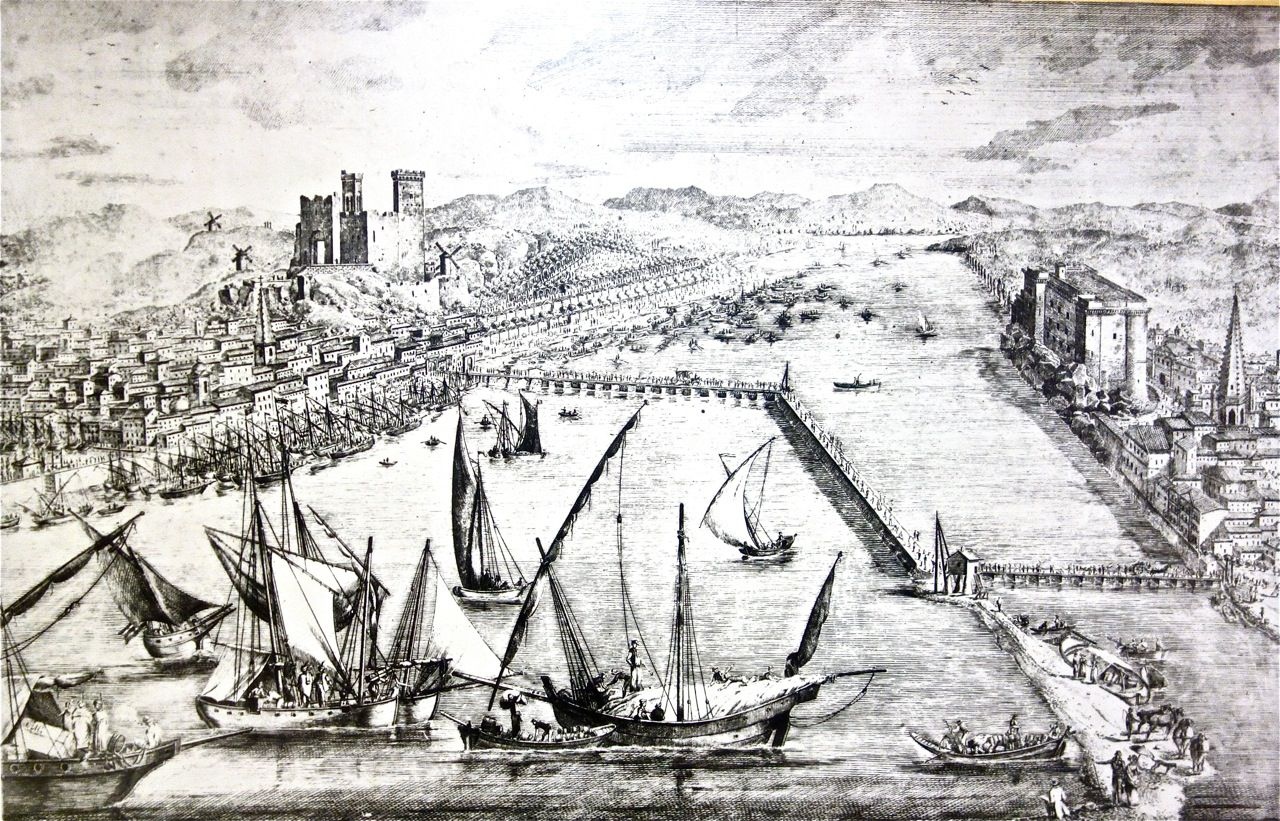
\includegraphics[width=1\linewidth]{Figures/foire5.jpg}
            	\caption{}
           		\label{subfig:foire2}
            \end{subfigure}
\caption{(a) "Vue de la foire de Beaucaire avec une partie de la ville de Tarascon", Basset André (1749). On distingue la ville de Beaucaire sur la droite et Tarascon sur l'autre rive. 
(b) Pont de bateaux reliant Beaucaire à Tarascon lors de la foire, auteur inconnu (XVIII\textsuperscript{ème} siècle). Le pont était alors régulièrement détruit lors des crues, empêchant toute communication entre les deux villes.}
\label{fig:foire}
\end{figure}

\section{Hydrométrie du Rhône à Beaucaire de 1816 à aujourd'hui}

	\subsection{Contexte hydrologique et hydrométrique}
	
	\paragraph{} Le Rhône à Beaucaire draine un bassin versant de 95 590 km² et son module est de 1680 m\textsuperscript{3}/s (1920-2023) (REF hydroportail). Beaucaire est la station hydrométrique la plus à l'aval du Rhône "complet", située 5 km à l'aval la confluence avec le Gardon (le dernier affluent du Rhône) et 10 km à l'amont de la diffluence qui donne naissance au Petit-Rhône et au Grand-Rhône (figure \ref{fig:BV}). Il s'agit donc de la station mesurant le débit le plus important du fleuve, mais également de France, le Rhône étant le premier fleuve français en terme de débit (à l'exception du Rhin qui est frontalier). Au delà de son important débit, le Rhône est un fleuve complexe de par la diversité de ses apports, comme décrit par \citet{parde_regime_1925} : "Dans une infinité de nuances et de contrastes, la Massa, l'Arve, l'Isère, la Durance, l'Ain, la Saône, l'Ardèche, c'est-à-dire des cours d'eau appartenant à toutes les catégories qu'on puisse trouver en Europe occidentale. [...] Ainsi, c'est par une carrière agitée que le petit torrent glaciaire de Gletsch devient le fleuve majestueux de Beaucaire, tour à tour ou en même temps nival et séquanien, océanique et méditerranéen, pondéré ou sujet aux plus déconcertants accès de démence". A Beaucaire, les signatures des affluents alpins, océaniques, méditerranées et cévenols se mélangent pour donner naissance à un régime hydrologique qu'il est difficile de classer dans une catégorie (figure \ref{fig:Regime}). Il en est de même pour ses crues, qui sont le reflet de la complexité de ses apports : "Il est violent par son courant encore inapaisé tout près de la Méditerranée, par ses crues de plus en plus nombreuses, désordonnées et massives, à mesure qu'il approche du terme de son cours" \citep{parde_regime_1925}. 


DESCRIPTION INSTRUMENTATION EN 2 STATIONS ET HISTORIQUE BCR

	\begin{figure}[h]
	\centering
		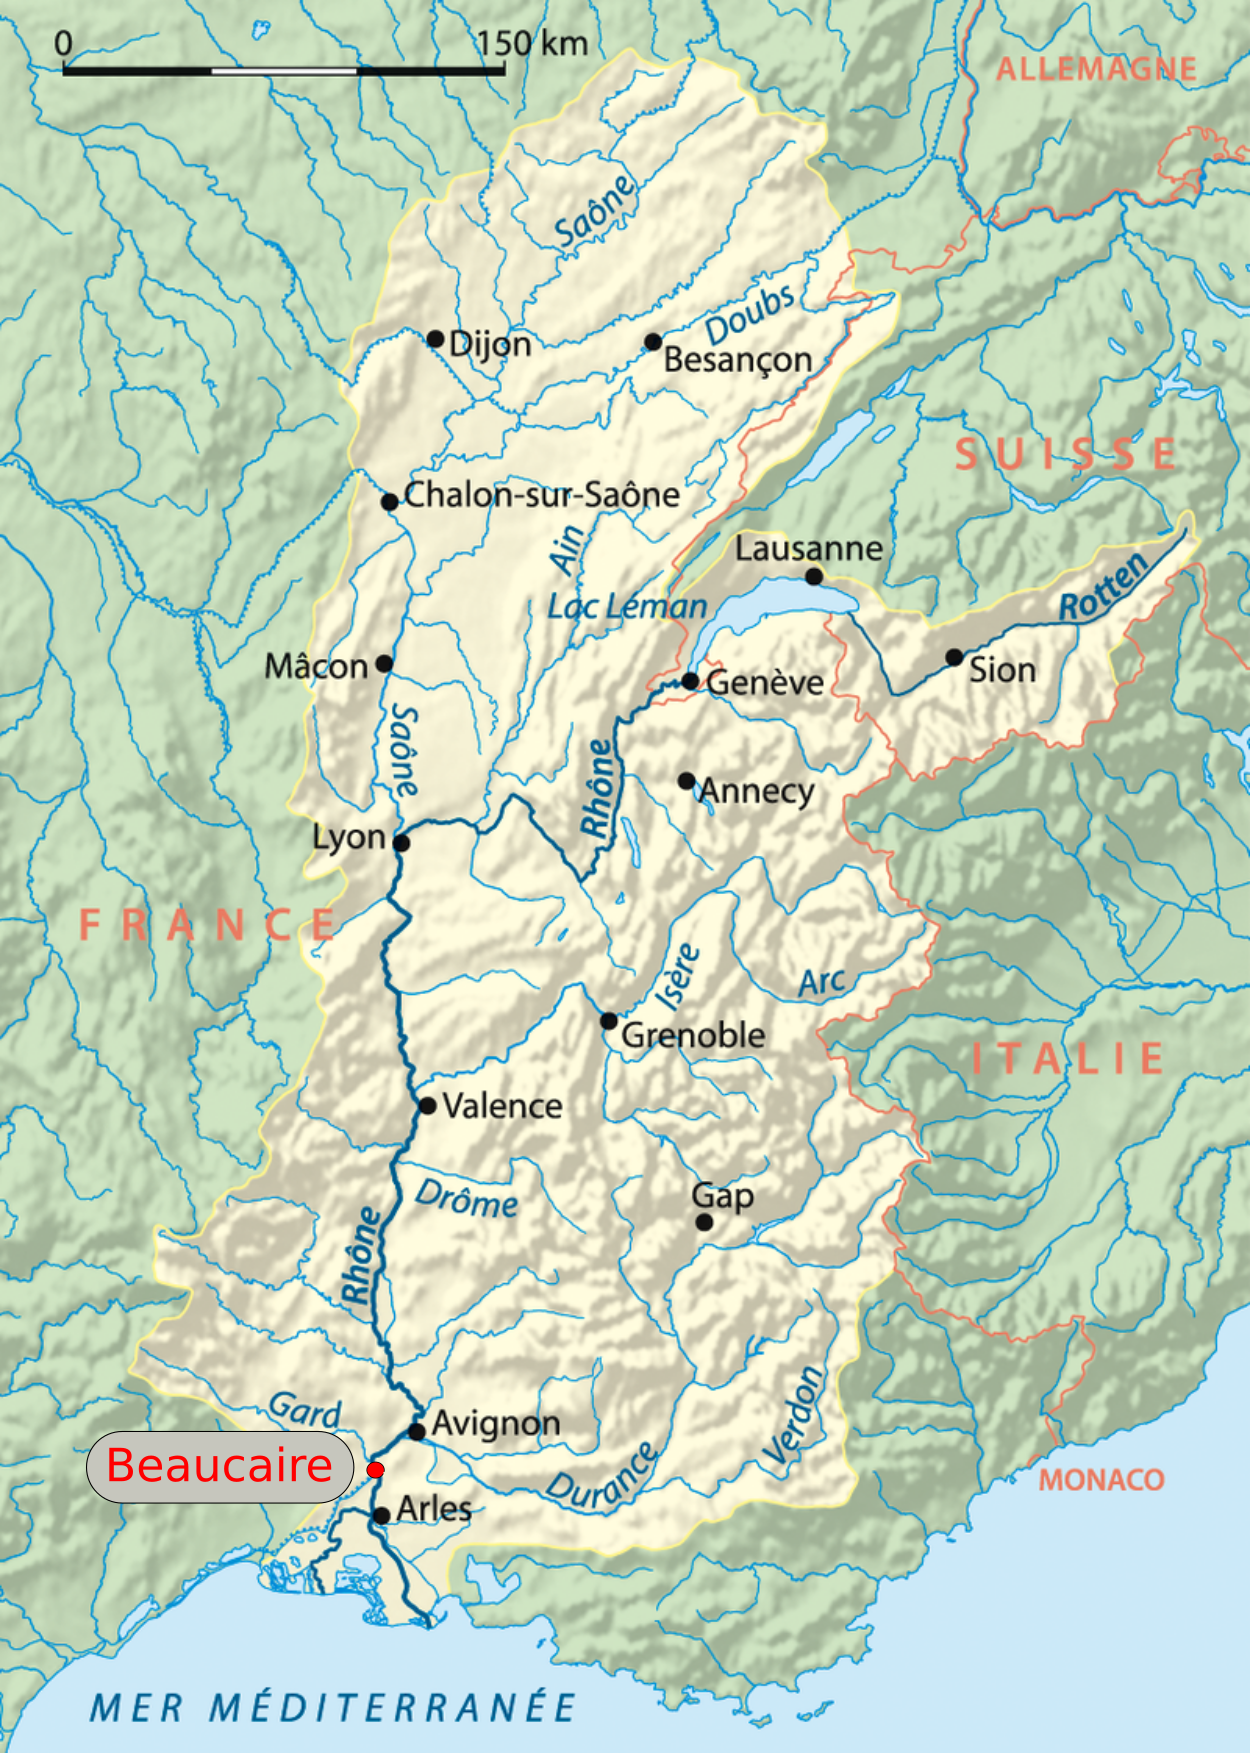
\includegraphics[width=.6\linewidth]{Figures/Rhone_bassin_versant.png}
        \caption{Bassin versant du Rhône. La ville de Beaucaire est indiquée en rouge (www.openstreetmap.org)}	
		\label{fig:BV}
	\end{figure}
	
	\begin{figure}[h]
	\centering
		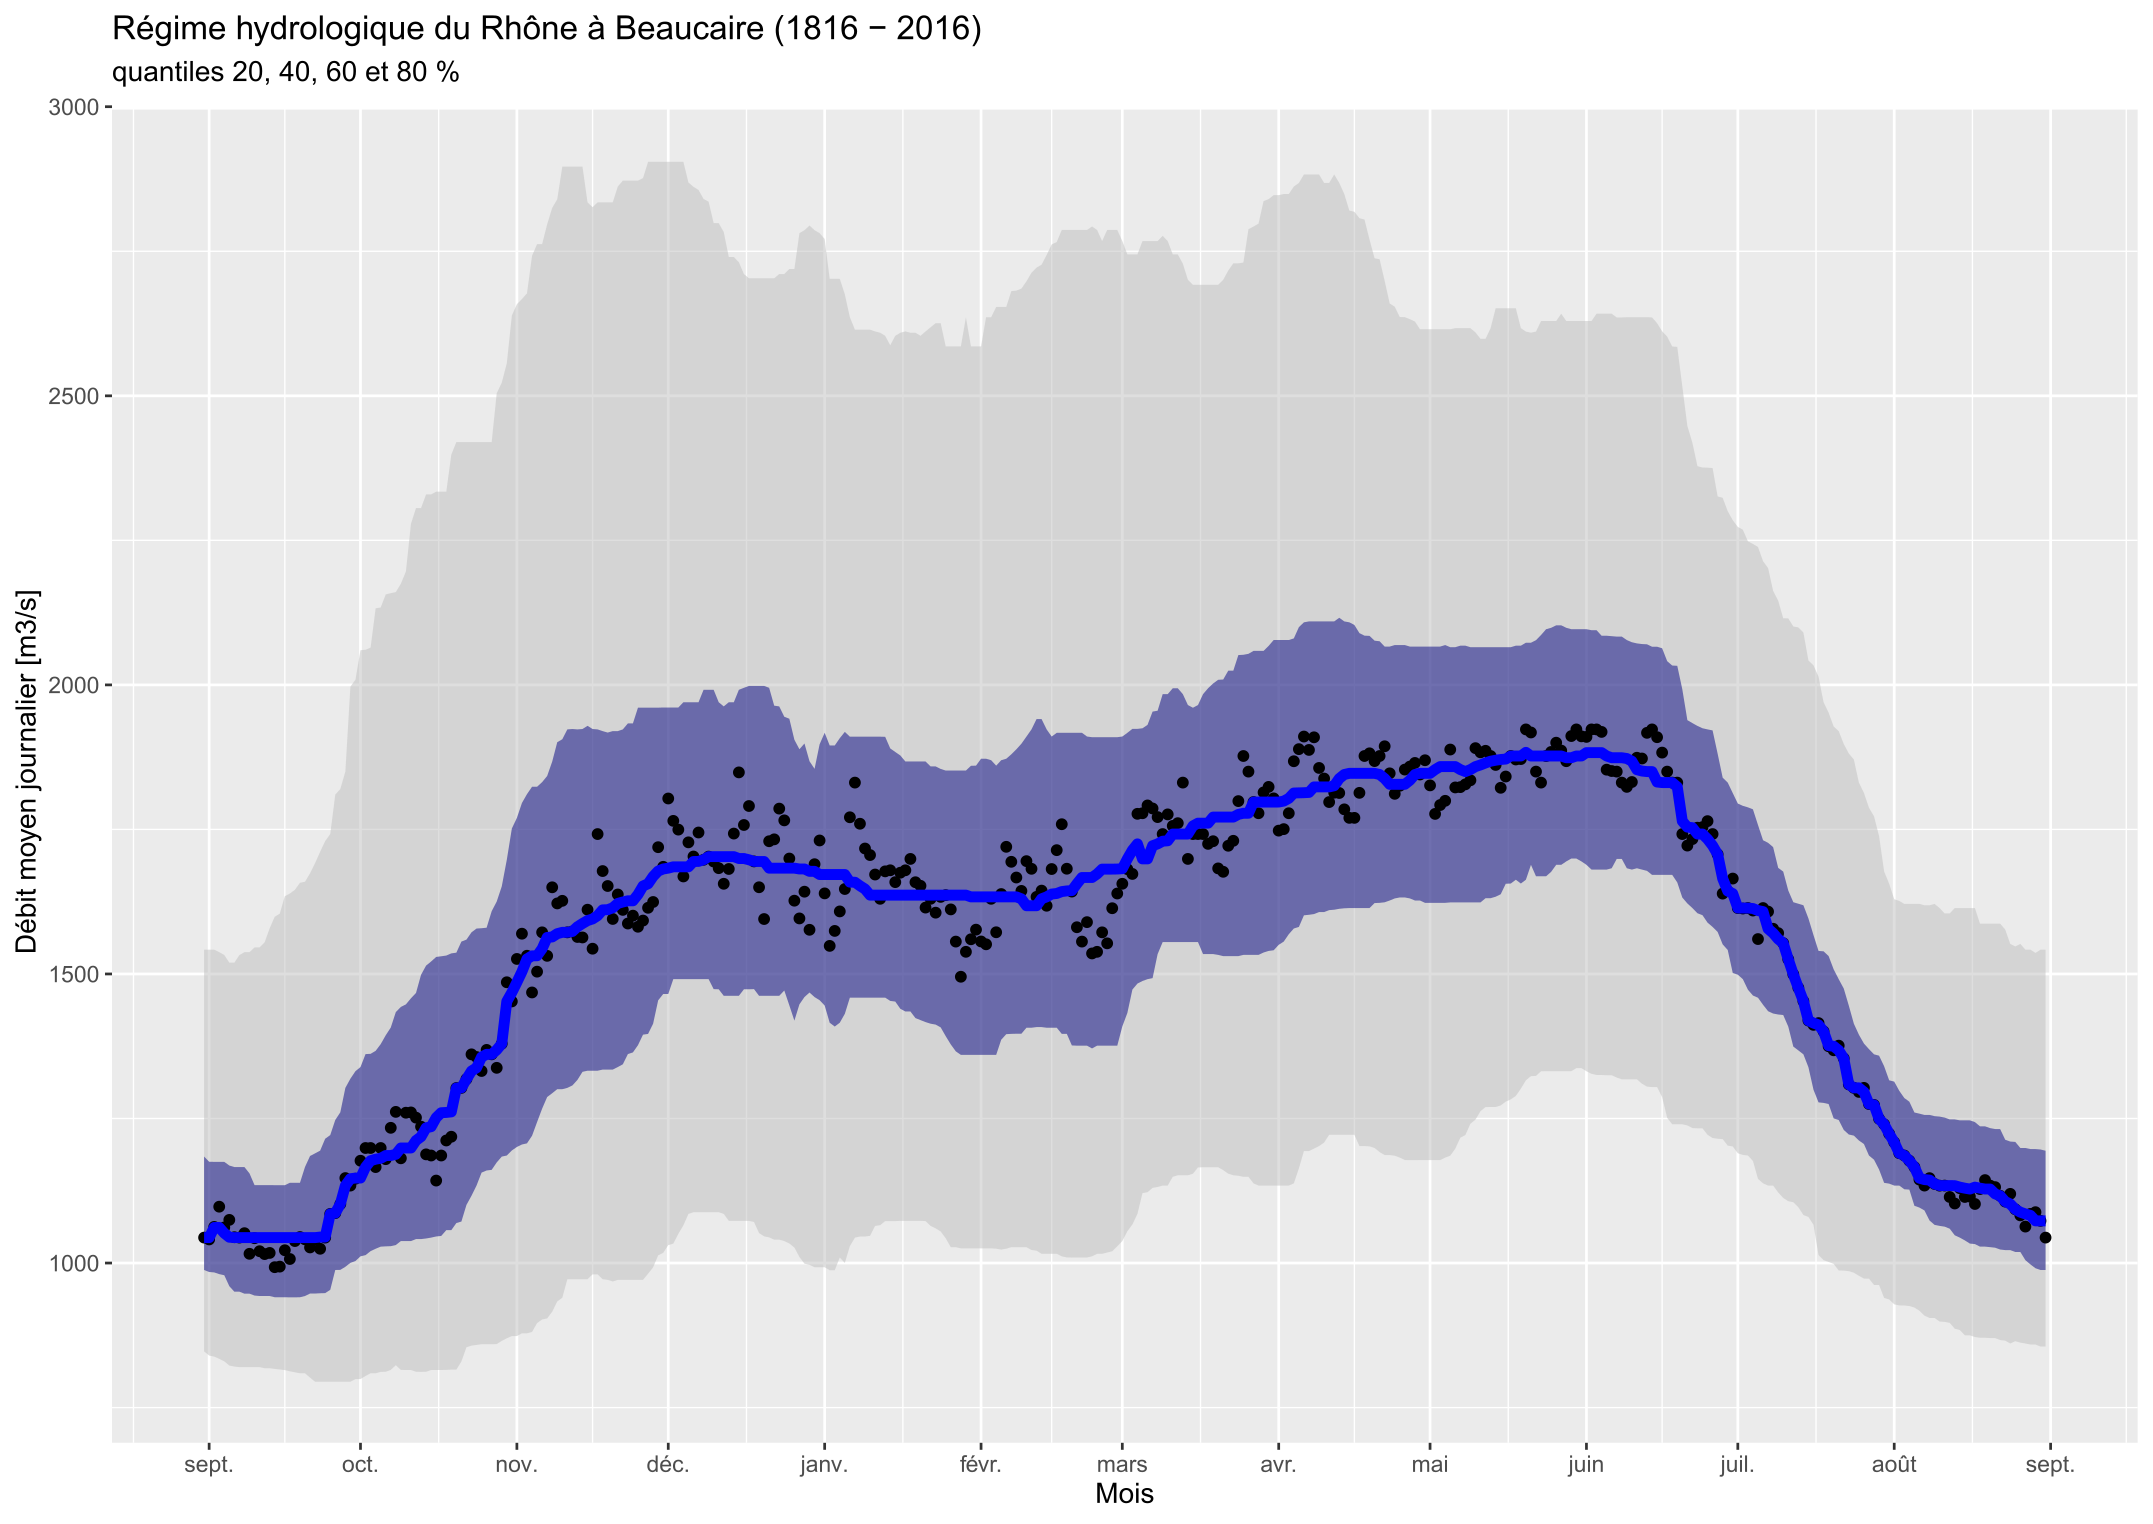
\includegraphics[width=.8\linewidth]{Figures/RegimeModif.png}
        \caption{Débit moyen journalier du Rhône à Beaucaire (1816-2016). En bleu foncé, les quantiles 40 et 60\%, en gris les quantiles 60 et 80\%.}	
		\label{fig:Regime}
	\end{figure}
	
	
\FloatBarrier

	\subsection{Station hydrométrique du Rhône à Pont de Beaucaire (1816-1967)}
	
	\paragraph{} Le travail d'archives de \citet{pichard_les_1995} et \citet{pichard_hydro-climatology_2017} a permis de reconstituer une chronique continue d'observations de la hauteur d'eau du Rhône à Beaucaire à partir du 15 Mai 1816 (tableau \ref{tab:MesuresPtBcr}). Ces relevés semble être les plus anciens qu'il soit possible de retrouver à Beaucaire (\citet{pichard_les_1995}; \citet{parde_regime_1925}). L'échelle limnimétrique fut installée sur le musoir de l'écluse du canal de Beaucaire à la mer (au point kilométrique 267.7), dont les travaux furent achevés en 1811. \citet{pichard_hauteurs_2013} souligne que "la longévité et la stabilité de cette échelle est évidemment exceptionnelle pour le bas Rhône. [...] La documentation chiffrée y est aussi précieuse et abondante qu'à Arles, mais cependant toujours aussi dispersée et accessible la plupart du temps par copie et non par les feuilles d'observations originales que les organismes gérants n'ont pas su conserver, en raison de transferts permanents d'attributions". Il faut noter que l'écluse du canal de Beaucaire fut remplacée entre 1914 et 1918 par une autre écluse débouchant plus à l'aval. Il semble cependant que le musoir que l'on observe de nous jours existait dès l'origine du canal et que l'échelle n'a subi aucun déplacement (\citet{pichard_hauteurs_2013}; \citet{bard_actualisation_2018}). 
	
	\begin{figure}[h]
	\centering
		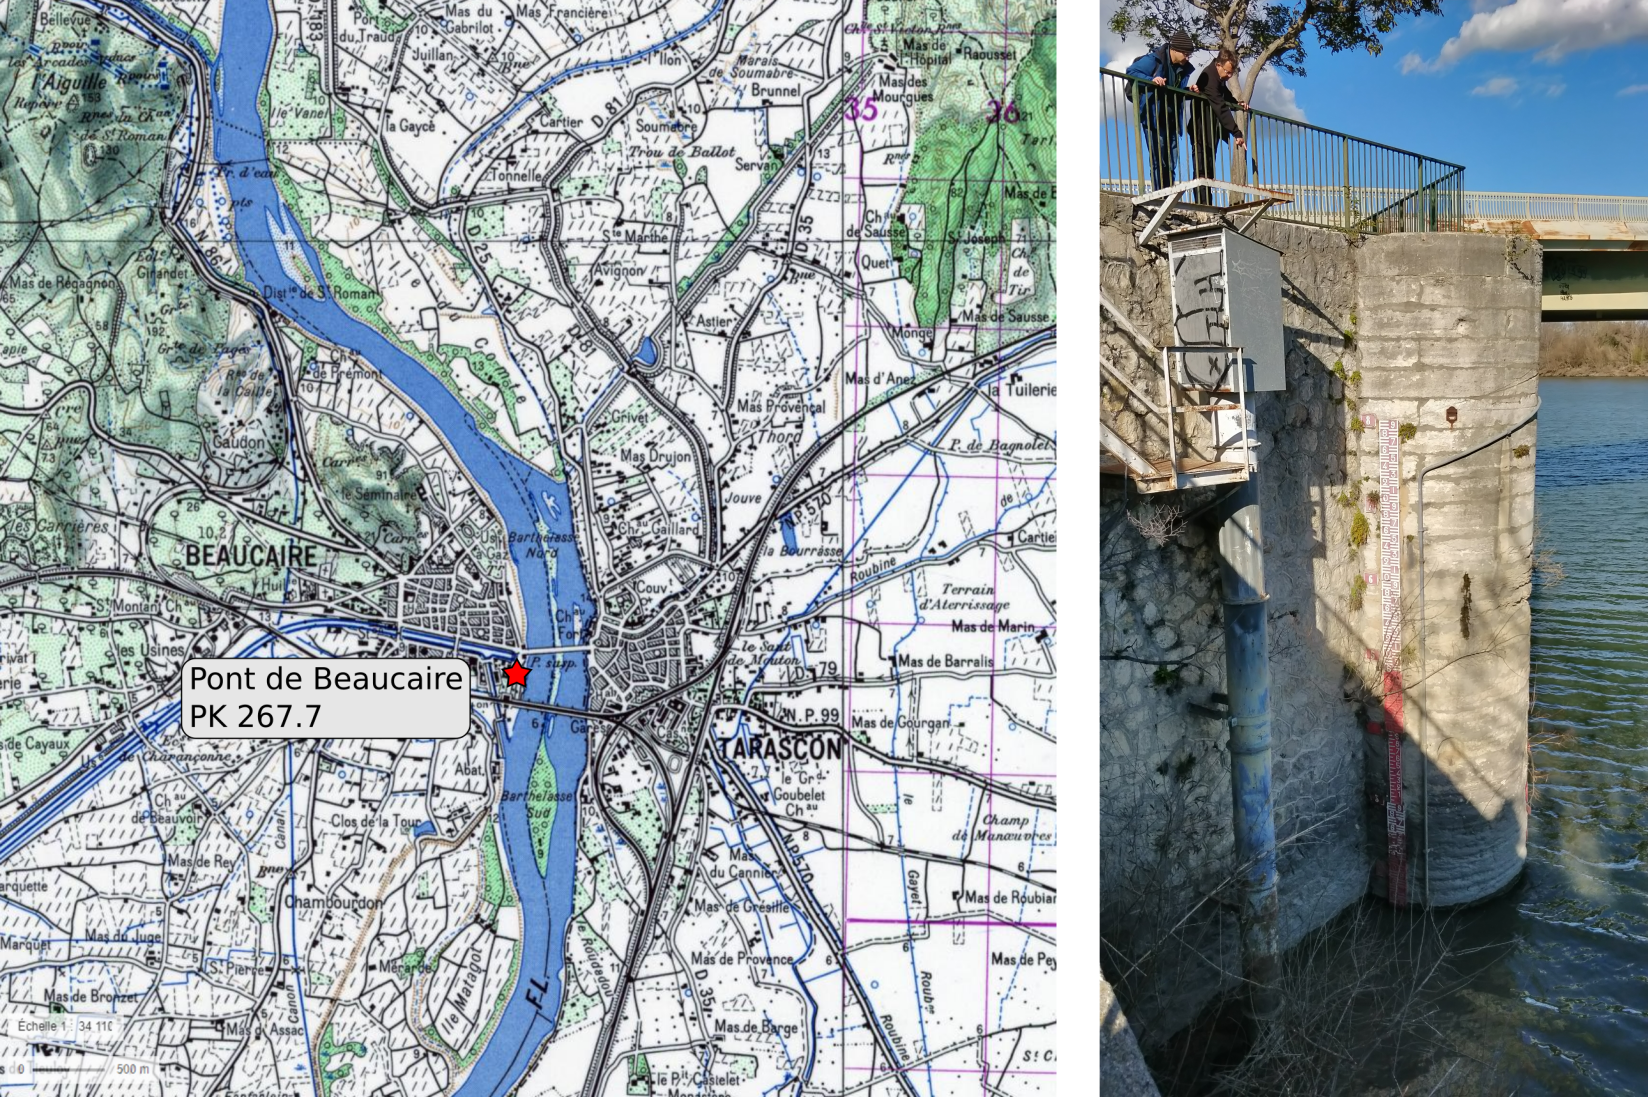
\includegraphics[width=.7\linewidth]{Figures/PtCartoPhoto.png}
        \caption{(Gauche) Localisation de la station de Pont de Beaucaire (carte IGN 1950, source : www.geoportail.fr). (Droite) Échelle et limnigraphe CNR de Pont de Beaucaire en Février 2020.}	
		\label{fig:CartoPt}
	\end{figure}
		
	\subsubsection{Relevés disponibles}
	\paragraph{} Les relevés retrouvés correspondaient probablement à une lecture d'échelle quotidienne en milieu de journée. Après la crue généralisée de 1840 et la création du Service Spécial du Rhône, une norme de trois relevés par jour (à 7h, 12h et 17h) se met lentement en place (figure \ref{fig:RelevesPt}). L'application de cette norme n'est visible dans les données qu'à partir de 1887, et ce jusqu'à la fin de l'exploitation de la station.  L'année 1967 marque le début des travaux d'aménagement de l'ouvrage hydroélectrique de Vallabrègues et de son canal de dérivation réalisés par la Compagnie Nationale du Rhône (CNR). Cette dérivation étant restituée à l'aval de la ville de Beaucaire, la station est déplacée 2 km plus à l'aval, environ 600 m à l'aval de la restitution des débits transitant par la centrale hydroélectrique. La nouvelle station, exploitée par la CNR à partir de 1970, sera alors appelée "Beaucaire Restitution".
	
	\begin{figure}[h]
          \centering
            \begin{subfigure}{0.49\linewidth}
            \centering
            	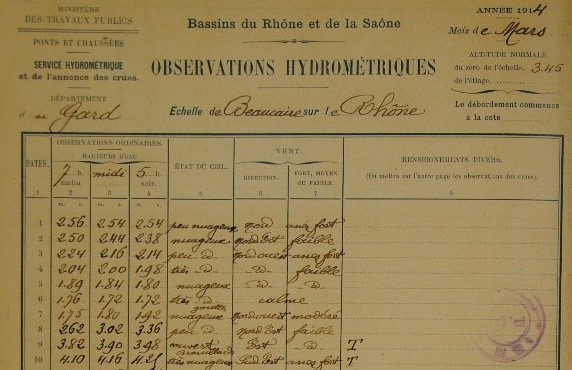
\includegraphics[width=1\linewidth]{Figures/TabObsBcrSmall.jpg}\hfill
            	\caption{}
            	\label{subfig:TabObsPt}
            \end{subfigure}
            \begin{subfigure}{0.49\linewidth}
            \centering
            	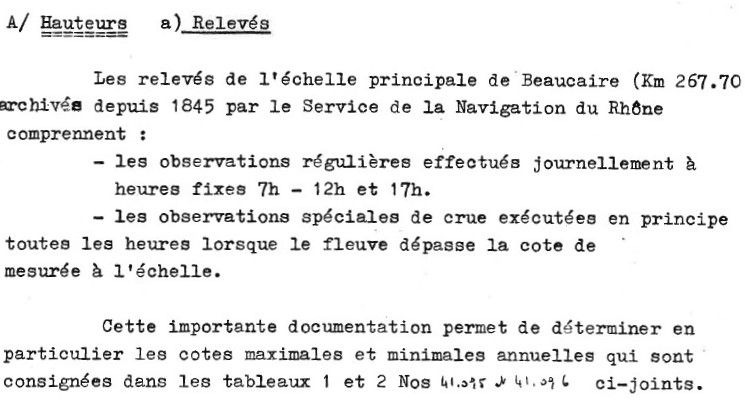
\includegraphics[width=1\linewidth]{Figures/RegleStationCNR}
            	\caption{}
           		\label{subfig:RegleCNR}
            \end{subfigure}
      \caption{(a) Feuille originale des relevés de hauteur d'eau à Beaucaire réalisés par le service spécial du Rhône en Mars 1914. On remarque les trois relevés par jour ainsi que des précisions sur l'état du ciel ou le vent. (b) Règles d'exploitation de la station de Pont de Beaucaire, fiche station de la CNR. On remarque que des observations horaires sont effectuées en crue mais la cote est effacée sur ce document (Source : Archives CNR, 1962)}
	 \label{fig:RelevesPt}
		
	\end{figure}            
            
    
	\begin{table}[h]
	\centering
	\caption{Détail des données de la station de Pont de Beaucaire (PK 267.7)}
    \label{tab:MesuresPtBcr}
	\resizebox{\columnwidth}{!}{%  
       \begin{tabular}{|c|c|c|c|c|c|} 
                \hline
               Période & Périodicité & Méthode & Origine & Zéro échelle & Commentaire \\
                \hline
                1816-1886 & 1 mesure/jour & Visuelle & 
                Service Spécial du Rhône & 3.34 mNGFo & Probablement mesure à 12h \\
                \hline
                1887-1967 & 3 mesure/jour & Visuelle & 
                Service Spécial du Rhône & 3.34 mNGFo & Relevés à 7h, 12h, 17h\\
                \hline
               1970-2020 & Horaire & Limnigraphe à flotteur puis LPN8 & 
                BD CNR & 0.03 mNGFo &  \\
                \hline
		\end{tabular}
		}
        \end{table}           
        
       
    \paragraph{} Les jaugeages les plus anciens récupérés dans les archives départementales du Rhône datent de 1845 (figure \ref{fig:Jau1845}) alors que les mesures limnimétriques débutent en 1816. Il faut noter que tous les jaugeages ont été effectués à l'amont de Beaucaire dans une zone plus stable et dépourvue d'îles (excepté les quatre jaugeages de 1845 et 1846, effectués au droit de la station de Pont de Beaucaire). Un total de 233 jaugeages est disponible à Pont de Beaucaire, couvrant la période 1845-1967, avec une fréquence peu homogène et des périodes non-jaugées (en période de guerre par exemple). 
    
    \begin{figure}[h]
	\centering
		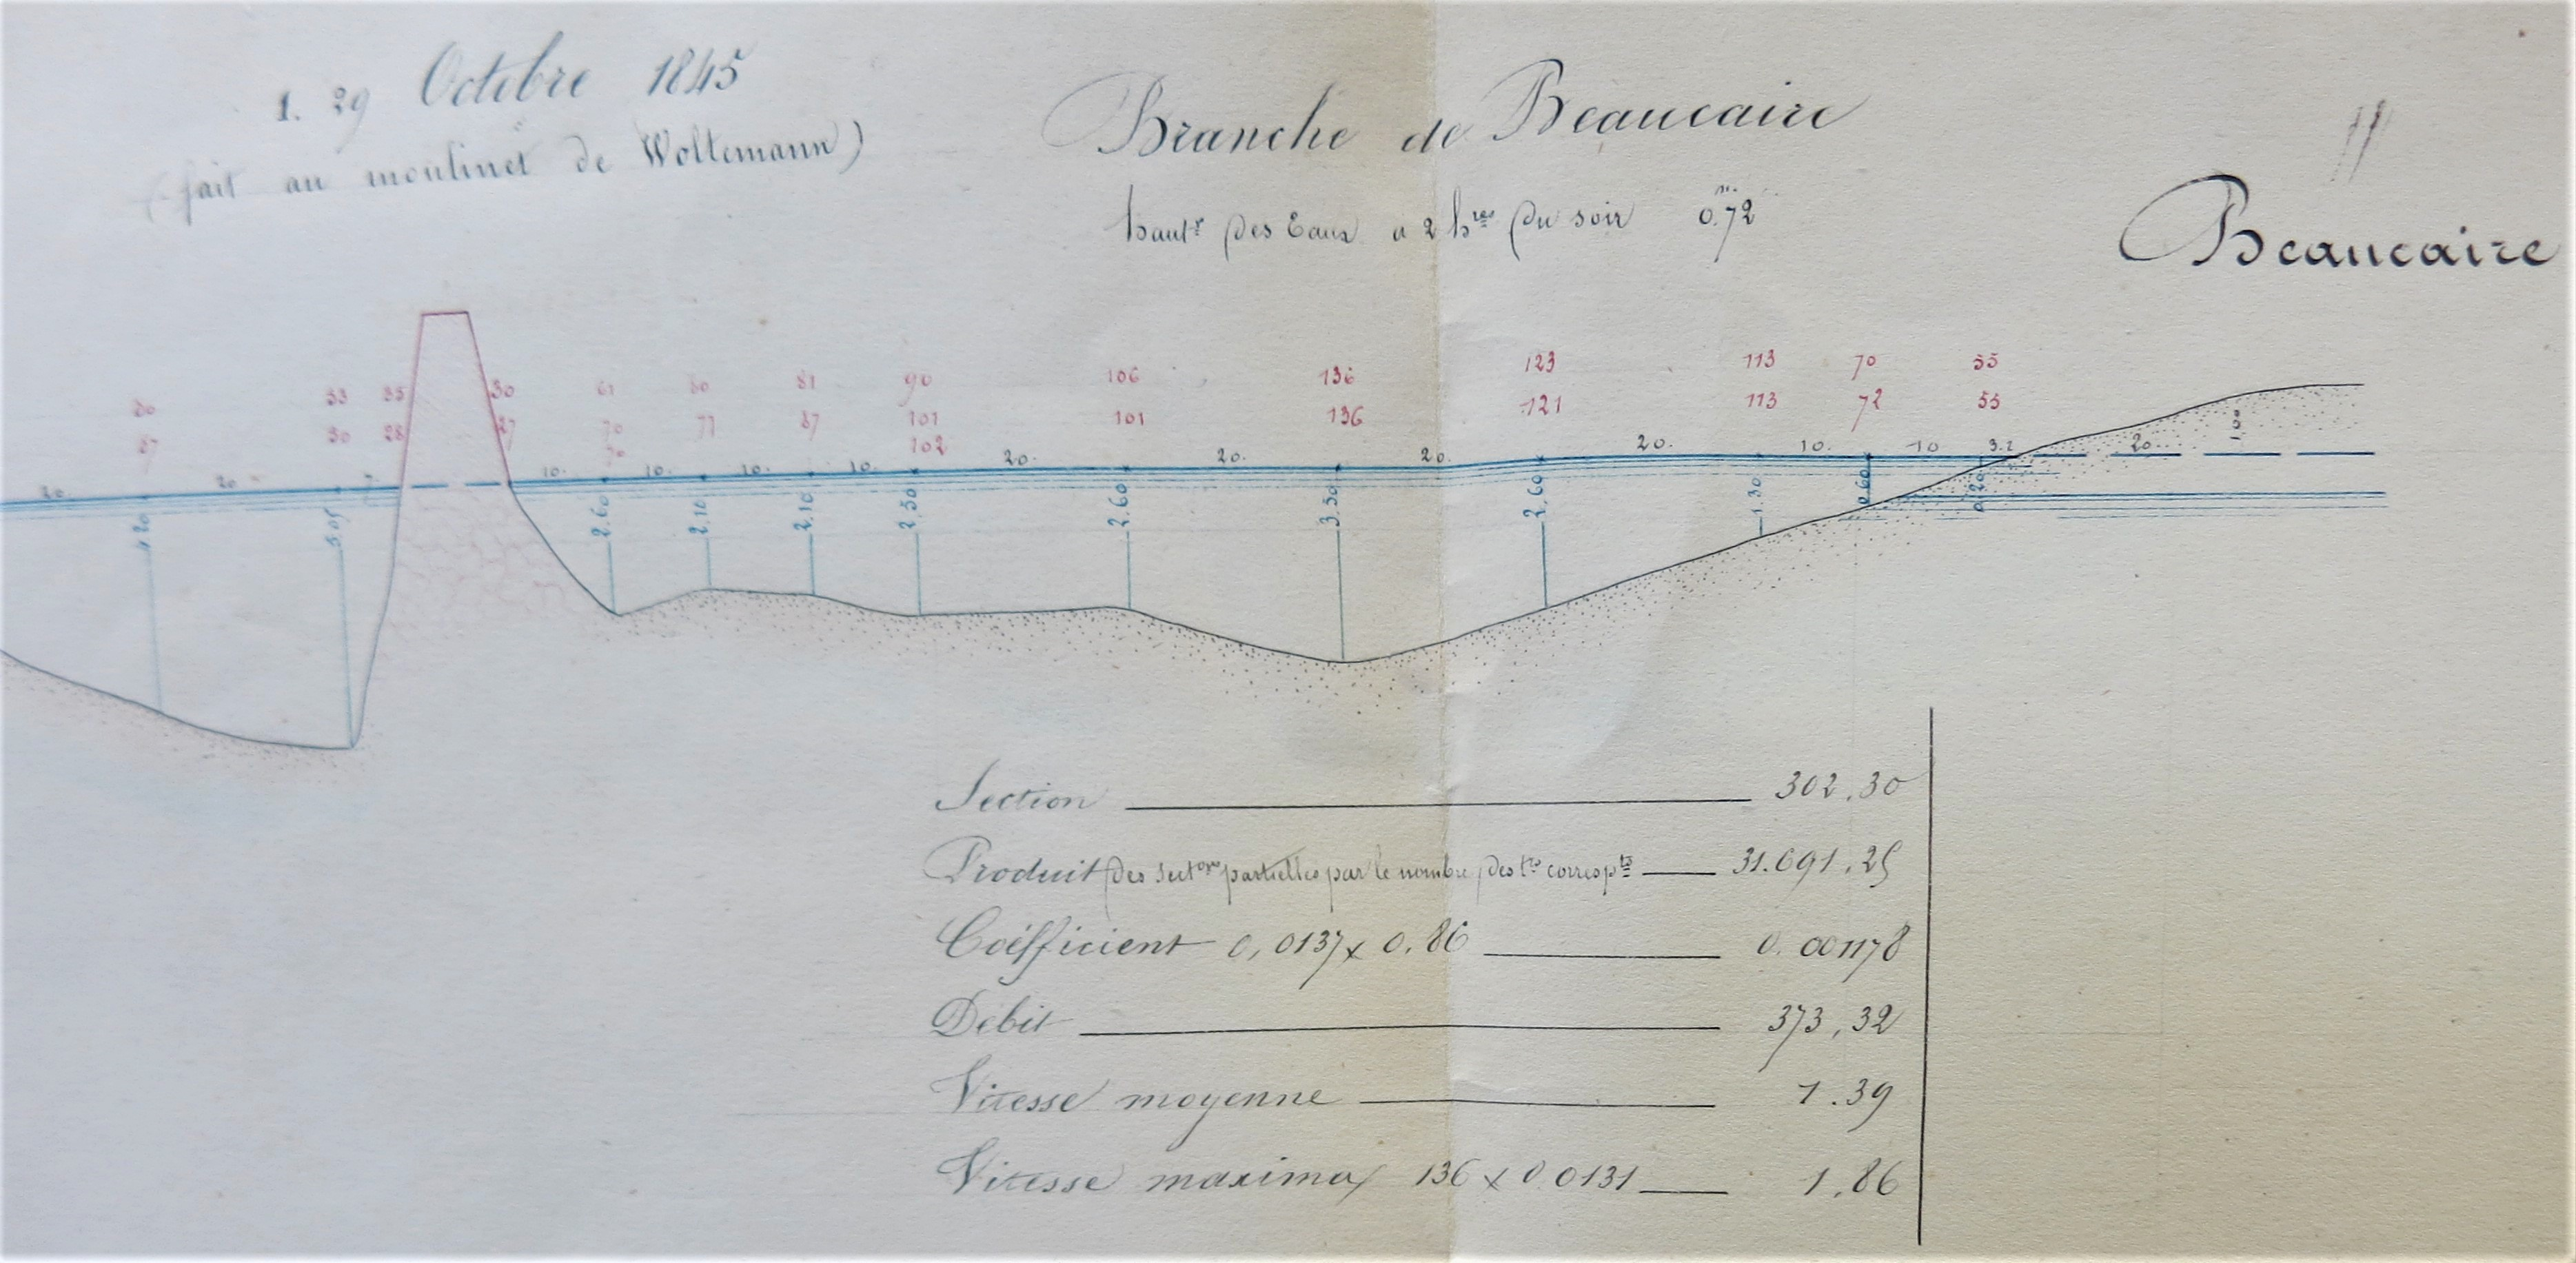
\includegraphics[width=.7\linewidth]{Figures/Jau1845.jpg}
        \caption{Jaugeage du 29 Octobre 1845 au droit de la station de Pont de Beaucaire, réalisé au moulinet de Woltmann par le Service Spécial du Rhône. En bas à droite, le détail du calcul du débit. Les chiffres en rouge représentent le nombre de tours du moulinet, probablement moyennés sur une verticale.}	
		\label{fig:Jau1845}
	\end{figure}
    
    Plot de l'ensemble des jaugeages disponibles?
	
	\subsubsection{Évolution de l'altitude du zéro de l'échelle}
    
    \paragraph{} Comme attesté par \citep{pichard_hauteurs_2013}, l'échelle limnimétrique de Pont de Beaucaire possède le rare avantage d'être restée à la même place depuis 1816, avec une altitude du zéro relativement stable dans l'histoire. Malgré les divers changements de référentiels altimétriques durant l'histoire, le zéro semble n'avoir que très peu varié (Tableau \ref{tab:zeroPt}). De la même manière que \citet{bard_actualisation_2018}, nous retiendrons la dernière mesure de la CNR qui semble être une valeur médiane de l'ensemble des valeurs connues : 3.37 m NGF IGN69 / 3.34 m NGF ortho (ou Lallemand). De plus, celle-ci est compatible avec les valeurs données lorsque la station était encore exploitée.

            \begin{table}[h]
                \centering
                \caption{Mesures de l'altitude du zéro de l'échelle à Pont de Beaucaire}
            	\label{tab:zeroPt}
                \begin{tabular}{| m{3cm} | m{3cm}| m{3cm} | m{3cm} |} 
                    \hline
                    Date & Altitude du zéro en m NGF IGN69 & Altitude du zéro en m NGFortho	& Organisme \\
                    \hline
                    1959 &	3.375 &	3.345 &	CNR\\
                    \hline
                    1961 &	3.36 &	3.33 &	CNR\\
                    \hline
                    2010 &	3.38 &	3.35 &	Symadrem\\
                    \hline
                    2010 &	3.37 &	3.34 &	CNR\\
                    \hline
            \end{tabular}
        \end{table}


\FloatBarrier
		\subsubsection{Travaux et aménagements}
    	\label{subsubsec:TravauxPt}
    
    \paragraph{} La largeur de la section du Rhône au niveau de Beaucaire (ou du moins, la largeur du lit majeur) n'a que peu évolué dans l'histoire car elle se situe au niveau d'un resserrement entre deux collines rocheuses. Ce resserrement est bien visible sur les champs d'inondation de 1840 et 1856 (Figure \ref{Champ1856}). En revanche, à une échelle plus réduite, de nombreuses modifications morphologiques, d'origine naturelle ou anthropiques ont pu affecter l'écoulement et modifier la relation hauteur/débit durant les deux siècles de relevés limnimétriques. Ces modifications sont listées dans les paragraphes suivants.
    
    \begin{figure}[h]
        \centering
        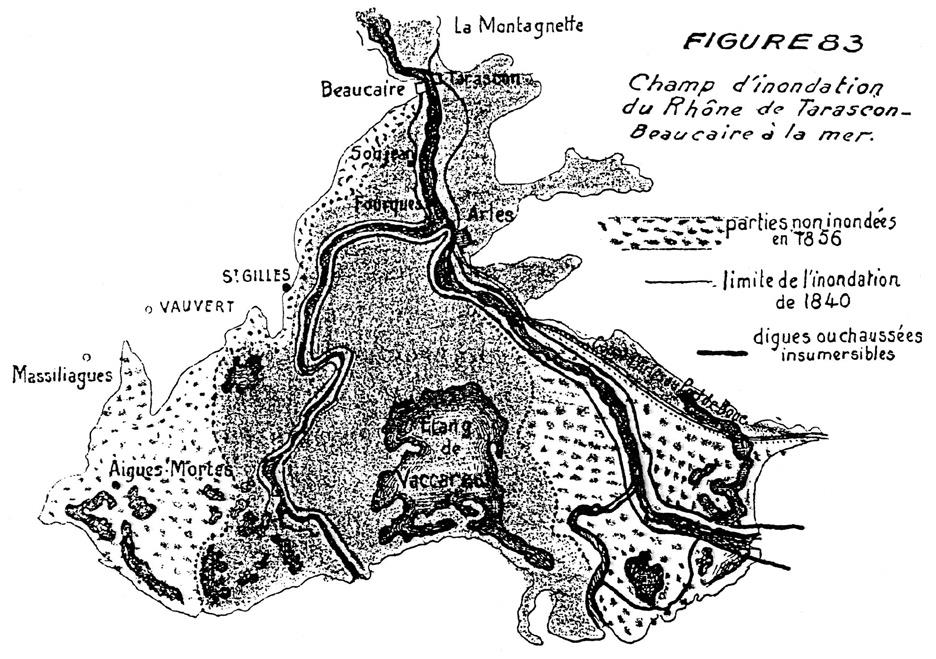
\includegraphics[width=.6\linewidth]{Figures/ChampInond1840-1856.jpg}
        \caption{Champ d'inondation du Rhône aval des crues de 1840 ou 1856, d'après \citet{parde_regime_1925}}
        \label{Champ1856}
    \end{figure}
    

	\paragraph{} Le premier pont reliant Beaucaire à Tarascon date de 1829. Il s'agit d'un pont suspendu composé de 4 piles (d'après la carte d'état-major de 1840), situé environ 30 m à l'amont du pont actuel, soit environ 45m à l'amont de l'échelle limnimétrique. Quelques années plus tard, en Juillet 1852, était inauguré le viaduc de chemin de fer de Beaucaire. Il est situé environ 250 m à l'aval de la station. Par la suite, les seuls travaux qui ont eu lieu dans le secteur sont ceux de l'aménagement CNR de Vallabrègues, entre 1967 et 1970. Ils ont sonné la fin de l'utilisation de la station par la CNR, devenue non-significative de la totalité du débit du Rhône suite à la création du canal de dérivation de l'aménagement. On peut noter la construction du pont routier actuel, entre 1988 et 1990, 30 m à l'amont de l'ancien pont. 
        

        \paragraph{} Depuis l'époque des plus anciennes cartes et récits retrouvés à Beaucaire jusqu'à aujourd'hui, des bancs de sable et îlots de diverses formes et dimensions ont séparé l'écoulement en deux bras plus ou moins distincts selon les périodes. De tout temps, mais pour des hauteurs d'eau différentes, les deux bras ont communiqué, un bras prenant le dessus sur l'autre au gré des événements morphogènes. Petit à petit, ces îlots ont été fixés par des digues afin de faciliter la navigation dans la zone, pour finalement arriver à la situation actuelle de deux bras bien distincts (figure \ref{fig:CartoRes}), comme en témoigne la carte d'\citet{armand_ii_1907} (figure \ref{fig:DigArmand}) qui décrit les différentes étapes de cette séparation. 
        
         \begin{figure}[h]
            \centering
            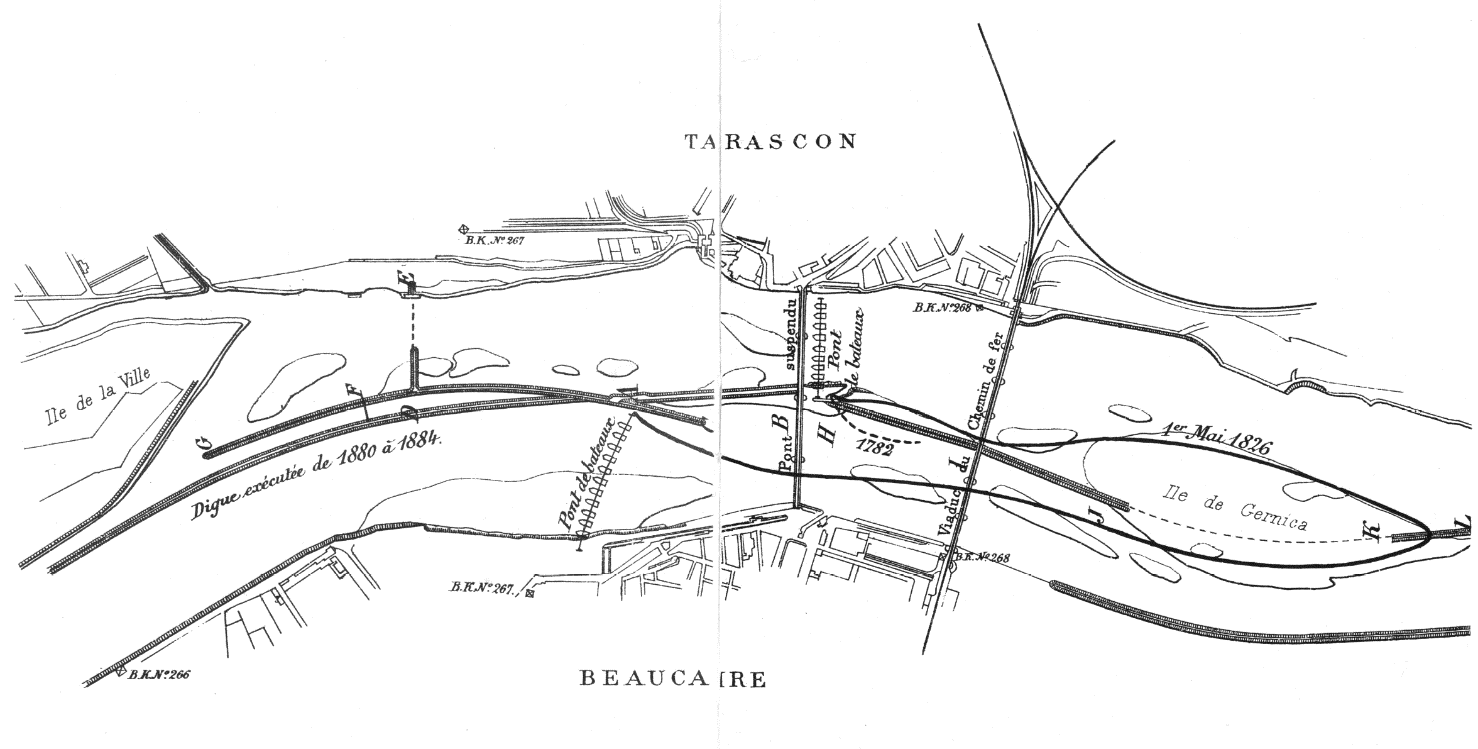
\includegraphics[width = 0.8\linewidth]{Figures/DiguesArmand.png}
            \caption{Carte de l'historique des digues de Beaucaire \citep{armand_ii_1907}}
            \label{fig:DigArmand}
        \end{figure}
        
        \begin{itemize}
            \item[$\bullet$] Digue divisoire (\textbf{AB}), antérieure à 1782
            \item[$\bullet$] Atterrissement (trait plein noir sur la carte) qui, dès 1826 se prolongeait jusqu'au point aval de l'île de Gernica. Il était probablement déjà présent au début du 19ème siècle.
            \item[$\bullet$] Érosion de l'île de la ville (à l'amont de Beaucaire) qui a modifié la répartition des débits entre les deux bras en faveur du bras de Tarascon. Pour maintenir la navigation dans le bras de Beaucaire, la digue \textbf{AB} fut prolongée à l'amont par une digue concave \textbf{CDF} en 1851 et par la suite, obstruction partielle du bras de Tarascon entre 1852 et 1855 \textbf{DE}. On peut constater cette érosion très rapide en faveur du bras de Tarascon sur les profils en travers de Goux (1850) (Figure \ref{fig:ProfGoux}). L'érosion de l'île de la ville peut être attribuée notamment à la crue catastrophique de 1840, possible déclencheur de ce phénomène.
            \item[$\bullet$] Forte érosion de l'atterrissement au niveau de \textbf{HI} du fait de l'écart de hauteur d'eau entre les deux bras pendant les crues. Une digue fut construite entre 1858 et 1859 pour pallier à ce phénomène.
            \item[$\bullet$] Pour ces mêmes raisons, construction d'une digue en aval du viaduc de chemin de fer \textbf{IJ} en 1872-1875 ainsi que la digue \textbf{KL} à l'aval de l'île de Gernica, qui se prolonge actuellement sur 2km vers l'aval.
            \item[$\bullet$] Prolongement de la digue concave \textbf{GF} autour de 1875
            \item[$\bullet$] Construction d'une nouvelle digue concave à l'amont de \textbf{GF} entre 1880 et 1884
        \end{itemize}

     
        
        \begin{figure}[h]
            \centering
            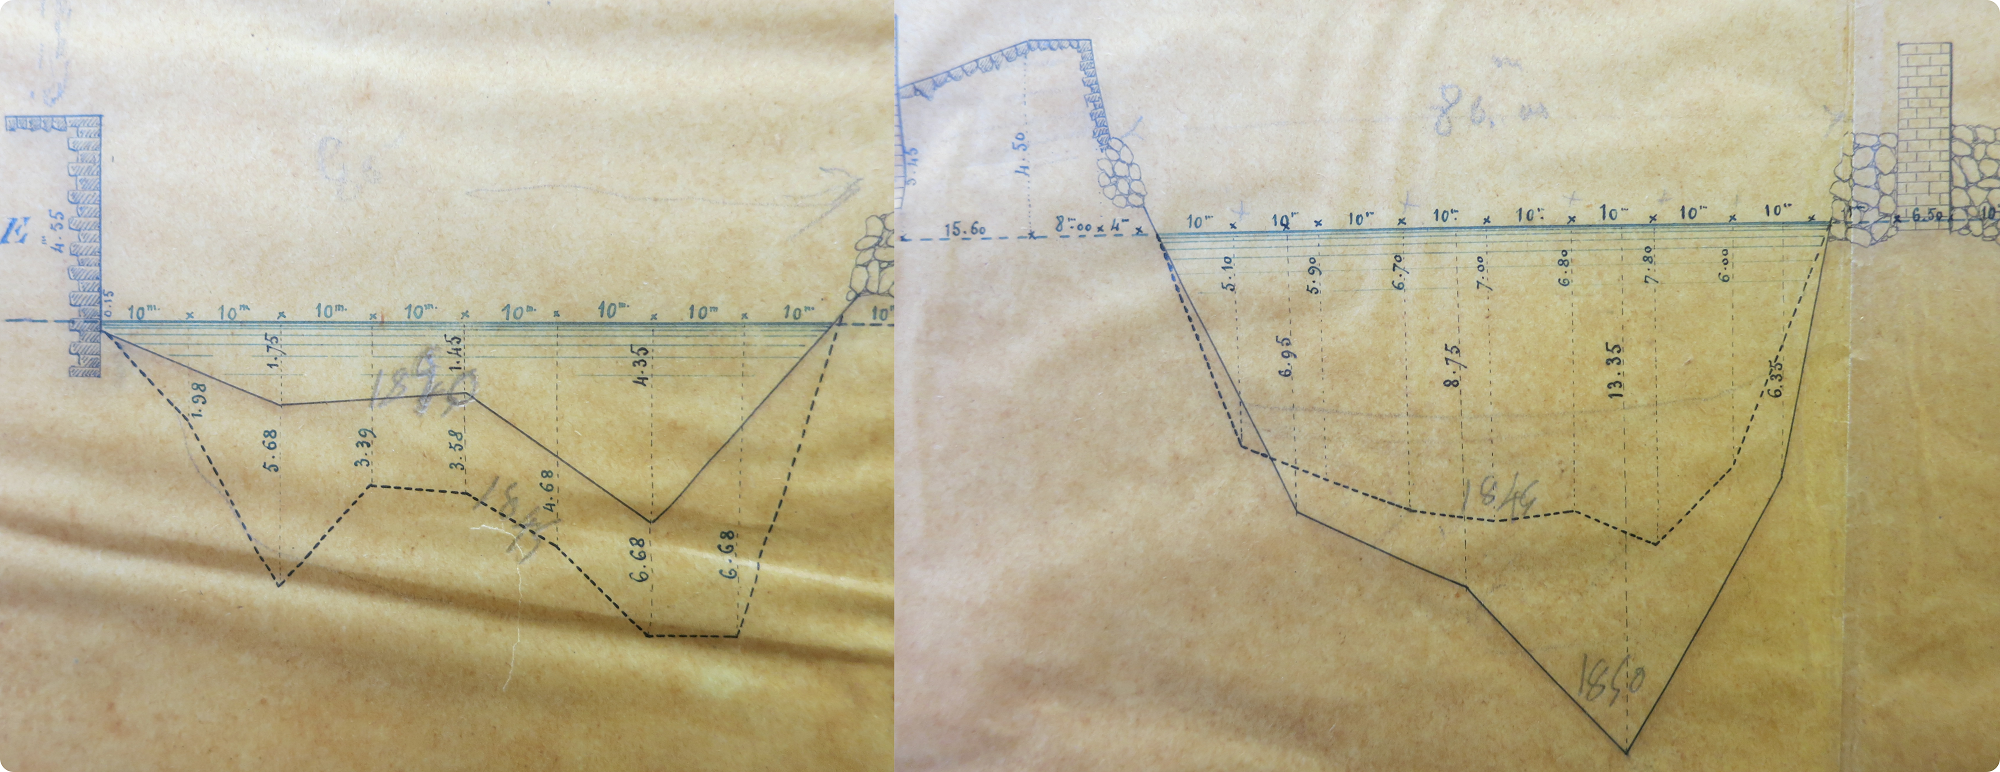
\includegraphics[width = 0.9\linewidth]{Figures/Goux4550.png}
            \caption{Profil en travers du bras de Beaucaire à gauche, et Tarascon à droite, en 1845 (pointillés) et 1850 (trait continu), \citet{goux_modification_1851}. On constate l'approfondissement du bras de Tarascon et le comblement du bras de Beaucaire.}
            \label{fig:ProfGoux}
        \end{figure}
            
        \begin{figure}[h]
            \centering
            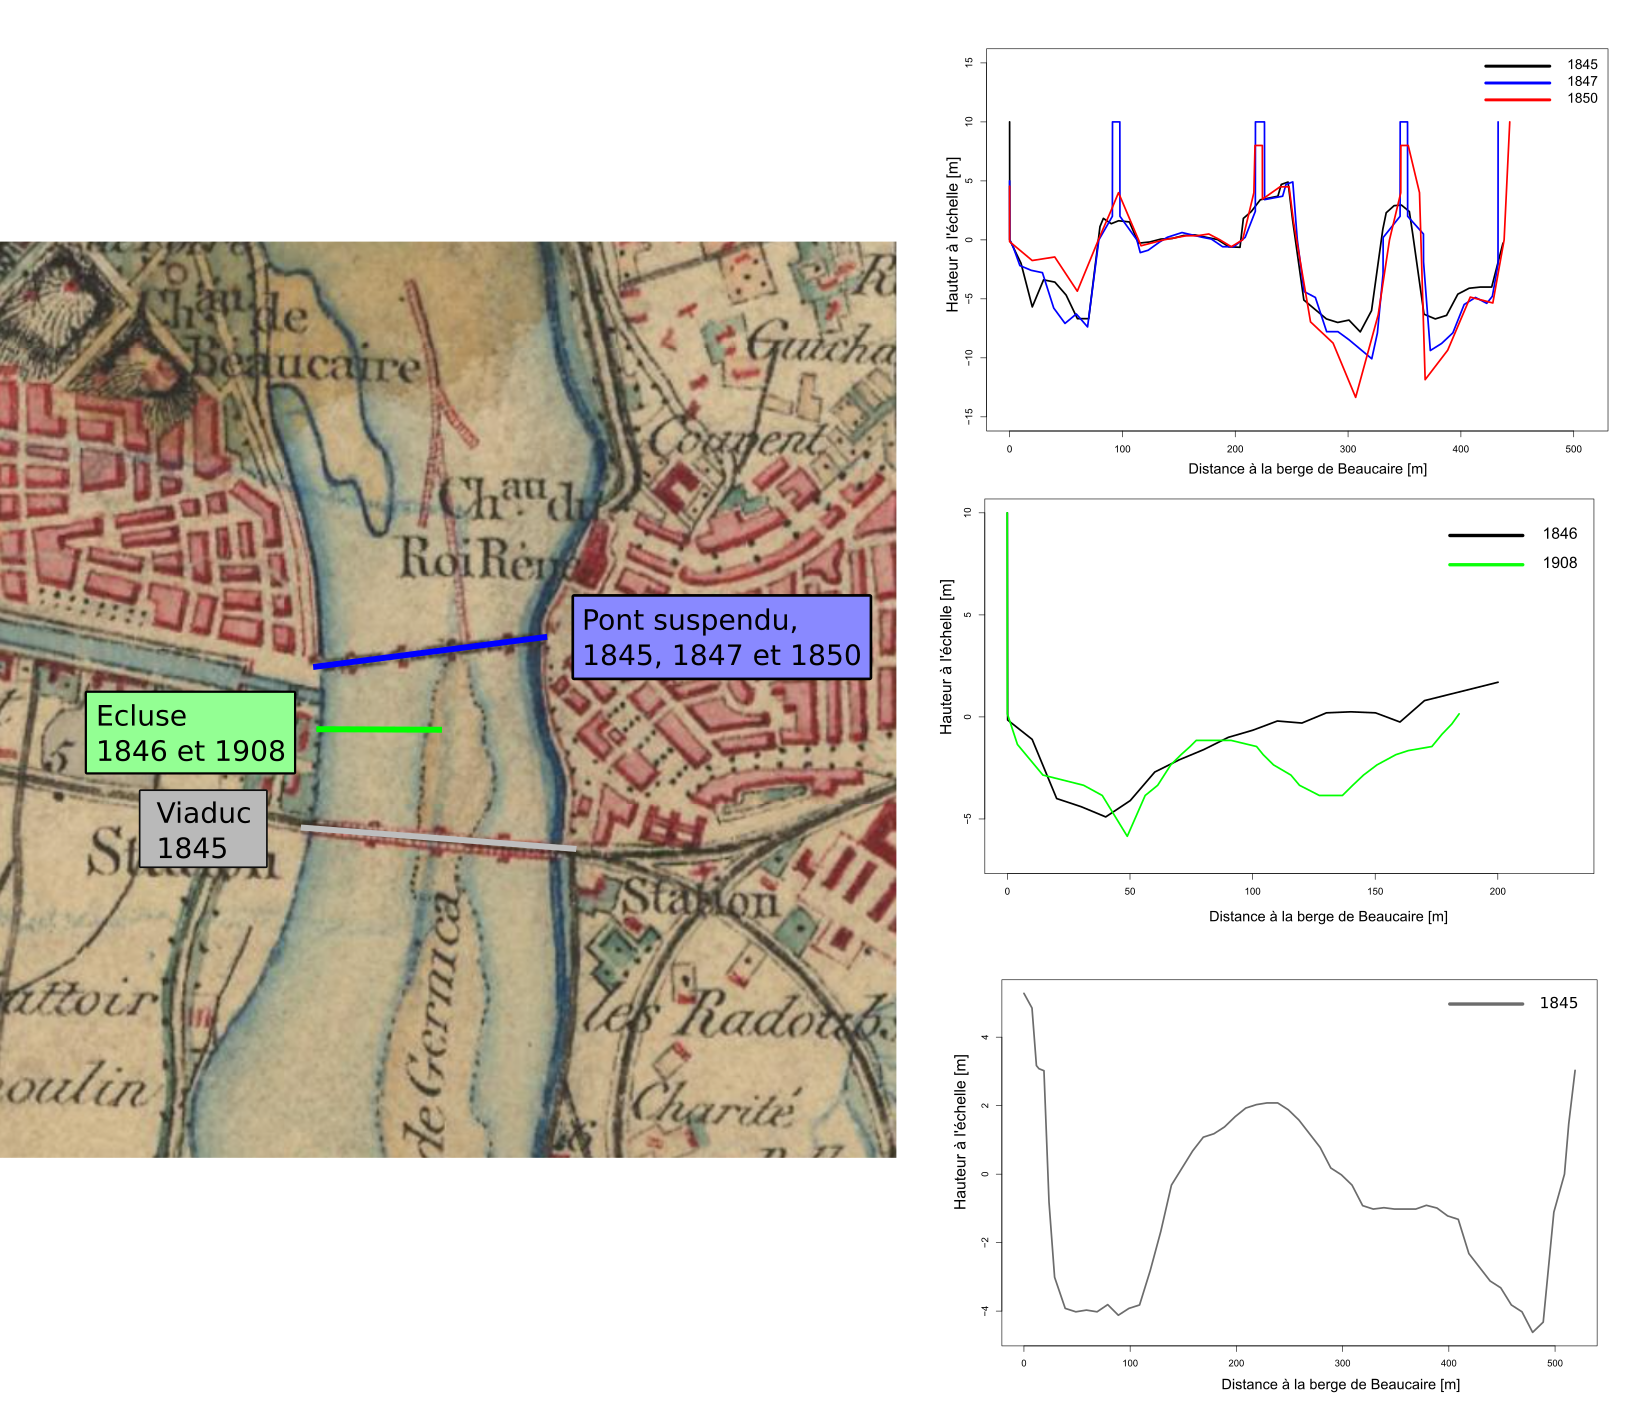
\includegraphics[width = 0.7\linewidth]{Figures/MapProfils.png}
            \caption{Profils en travers XIXème siècle}
            \label{fig:Profis19eme}
        \end{figure}
            
\FloatBarrier
        \paragraph{} Suite à la fixation des deux bras par les digues divisoires vers la fin du XIX\textsuperscript{ème} siècle, on peut supposer qu'il n'y a eu pratiquement aucun changement jusqu'au début des aménagements CNR de Vallabrègues (débutés en 1967 et mis en service en 1970), en témoignent les photos aériennes du portail " Remonter le temps " de l'IGN, de 1936 à 1947 (Figure \ref{fig:AerialBcr}). Ainsi, l'isolement quasi-total du bras de Tarascon au profit du bras de Beaucaire est finalisé en 1884 et a connu de nombreuses phases d'aménagement débutant vers la fin du 18ème siècle. Il est probable qu'à l'époque ancienne, tout comme aujourd'hui, les deux bras communiquaient à haut débit, certainement aux alentours de 6m à l'échelle à l'époque de la finalisation des digues, et à des hauteurs moindres auparavant. Certaines sources signalent par exemple qu'il était ponctuellement possible de traverser en bateau d'un bras à l'autre au niveau de la ville entre 1858 et 1872. Le bras de Beaucaire a sans doute été prépondérant sur le bras de Tarascon sur la majeure partie de l'histoire de la station, excepté la période 1840-1850, en témoignent les profils en travers de \citet{goux_modification_1851} (Figure \ref{fig:ProfGoux}).
    
        \begin{figure}[h]
            \centering
        	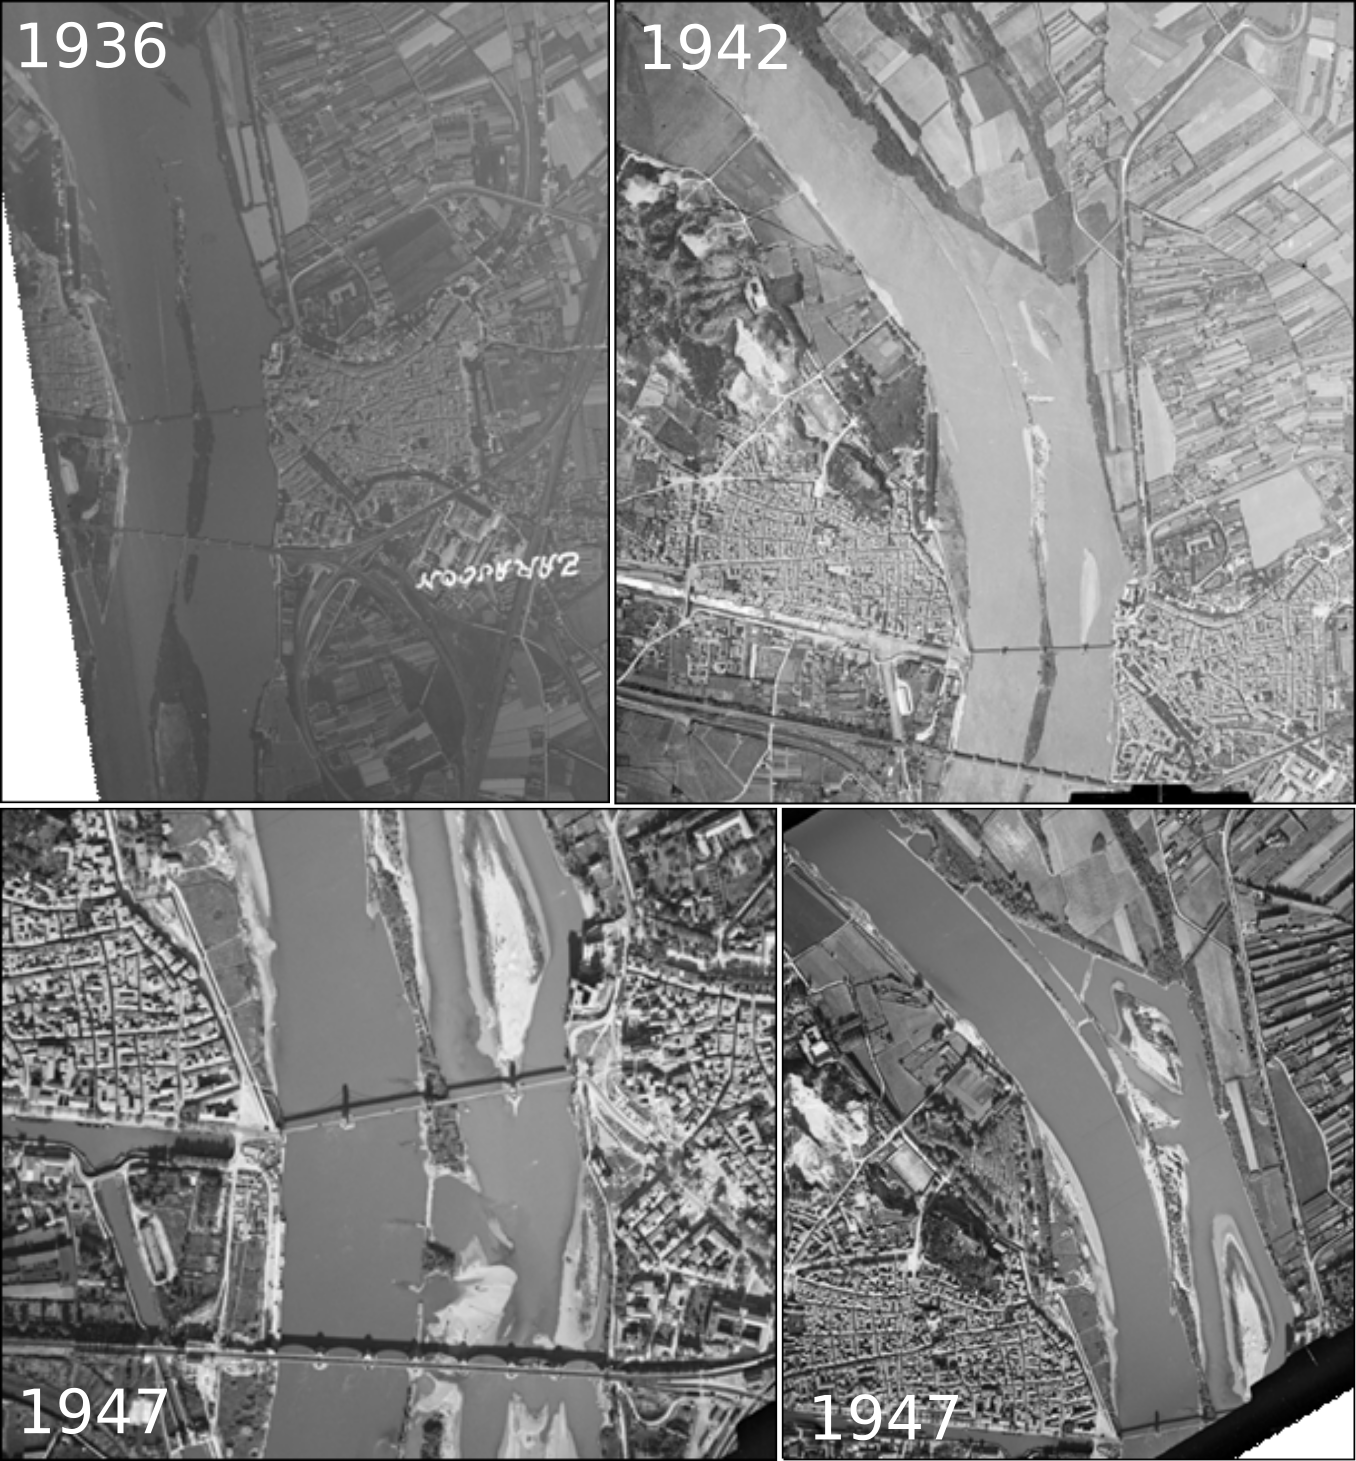
\includegraphics[width = 0.7\linewidth]{Figures/AerialBcr.png}
            \caption{Images aériennes du Rhône à Beaucaire entre 1936 et 1947 (source : www.géoportail.gouv.fr). On remarque la présence des digues sur les 4 images, particulièrement en 1947 pour des débits très faibles.}
            \label{fig:AerialBcr}
        \end{figure}
    
		\paragraph{} Au cours des décades 1860 et 1870, les travaux d'aménagement en lit mineur imaginés par l'ingénieur Girardon sont lancés. Ils permettront de favoriser la navigation fluviale en fixant les berges par l'installation d'épis noyés transversaux sur une grande partie du linéaire du Rhône français. Des épis ont été installés à l'amont et à l'aval de Beaucaire et ont probablement influencé la relation hauteur/débit au droit de la station.
    
		\paragraph{} Les désordres du Rhône à l'aval de Beaucaire étant réguliers avant son endiguement, on imagine que la création des digues a coïncidé avec l'installation des populations dans le secteur, comme attesté par \citet{surell_memoire_1847} : "Si l'on considère que l'existence de la plaine est presque inévitablement liée à celle des chaussées, on doit croire que celles-ci sont contemporaines de la civilisation même du pays, et qu'elles ont dû occuper, depuis longtemps, les soins de la population" (les digues étaient fréquemment appelées chaussée dans l'époque ancienne, car elles faisaient également office de voies de circulation). \citet{mejean_etude_2017}, cite l'ingénieur Girard, qui, en 1857, affirme que : "la construction des premières chaussées entre Beaucaire et Sylvéréal (Camargue) date de l'époque romaine. L'initiative personnelle des propriétaires a ensuite contribué à dresser un système de protection où chacun établissait une levée de terre pour se protéger des invasions du Rhône. La plupart de ces chaussées étaient établies sur les bourrelets alluviaux, car ils présentaient l'avantage d'être déjà surélevés par rapport aux terres voisines. Les chaussées ne présentaient pas une ligne continue de défense, les protections s'établissant autour de quelques grandes propriétés." Par la suite, plusieurs grandes phases d'aménagement des digues de protections se sont succédées. Avant le XVI\textsuperscript{ème} siècle, les aménagements étaient discontinus mais deviennent plus organisés avec l'essor de l'agriculture dans les plaines alluviales. Au début du XIX\textsuperscript{ème} siècle, un endiguement continu de Beaucaire à la mer est installé grâce à l'harmonisation des nombreuses associations ou "syndicats des digues", jusqu'alors "aussi multiples que rivales" \citep{pichard_sept_2014}. Il protège les populations pour les crues courantes, prétendument jusqu'à la décennale. Au niveau de Beaucaire, la digue de la Montagnette existant depuis le XV\textsuperscript{ème} siècle connut de nombreuses avaries en 1840, 1841, 1843. Des travaux de rehaussement furent effectués en 1843 ainsi qu'en 1883. La digue du chemin de fer (de Tarascon à Arles en rive gauche) vint remplacer en 1846 les digues historiques du Trébon, souvent rompues dans l'histoire. La digue du Trébon était élevée à 6.5 ou 7m au-dessus de l'étiage. La digue du chemin de fer est élevée à 2m10 au-dessus des plus hautes eaux connues à l'époque (1843). Lors de la rupture de la digue de la Montagnette en 1856, Tarascon était enfermée entre Montagnette et le remblai du chemin de fer, l'eau était ainsi restée dans les plaines pendant plusieurs semaines. Ces digues principales furent complétées par des aménagement au sein des villes de Tarascon et Beaucaire entre 1860 et 1866. La "banquette de Beaucaire", constituée d'un mur maçonné construit en 1840 du rocher du château à la chaussée de chemin de fer, fut rehaussée après 1856, puis en 1862 et 1863, environ 2m au-dessus du niveau atteint en 1856. Il en va de même pour les quais de Tarascon et de la digue de la Montagnette, rehaussés en 1860 à 1m50 au-dessus du niveau de 1856.
		
		\paragraph{} Ces nombreuses protections érigées au cours du XIX\textsuperscript{ème} siècle on permis de contenir les crues courantes, puis des crues plus importantes grâce aux aménagements postérieurs aux inondations de 1840 et 1856 qui furent à l'origine d'une prise de conscience illustrée par la création du Service Spécial du Rhône des Ponts et Chaussées. Depuis cette époque, les systèmes de protection n'ont que peu évolué et la crue de 2003 a ravivé les inquiétudes quant au risque de brèches, comme en témoigne cet extrait du rapport du \citet{symadrem_programme_2012} (Syndicat Mixte Interrégional d'Aménagement des Digues du Delta du Rhône et de la Mer) : "Le système actuel de protection contre les crues du Rhône a été réalisé après les grandes crues de 1840 et 1856. Il est ancien et présente une exposition très forte au risque de brèches. Dans l'état actuel, on estimque que le risque de formation de brèches, confirmé par les crues de 1993, 1994, 2002 et 2003, est quasi-certain à certain". Depuis la crue de 2003, un programme de sécurisation a été réalisé, prévoyant notamment la réalisation de digues résistantes à la surverse et à la formation de brèches (REF SYMADREM).    
		
		\subsubsection{Évolution géomorphologique}
		
		SECTION TIREE DE BARD ET LANG, A REVOIR
		
		\paragraph{} Il est évident que les conditions d’écoulement du Rhône ont varié depuis l’implantation de la station hydrométrique de Beaucaire. D’une part l’évolution naturelle du transport sédimentaire depuis la fin du petit Age glaciaire, et d’autres part les nombreux aménagements réalisés sur le fleuve au XIXème et XXème siècles : à la fois dans le lit mineur pour la navigation et la stabilisation des berges mais aussi dans la plaine d’inondation par l’érection ou le renforcement de digues contre les inondations, sans compter les modifications du transit sédimentaire sur le Rhône et ses affluents au gré des aménagements hydro-électriques.
La thèse menée par Guillaume Raccasi (2008) sur les mutations géomorphologiques du Rhône aval apporte de nombreux éléments qui sont ici repris pour éclairer l’évolution des conditions hydrauliques à Beaucaire :

\paragraph{} La plaine d’inondation entre les digues insubmersibles, homogénéisées dans les années 1850-90, affiche une stabilité globale sur une période de 150 ans (1876-2003). Entre Beaucaire et Arles les différences d’hydraulicité du lit majeur sur cette période sont minimes. En amont du défilé de Beaucaire, dans la plaine de Vallabrègues-Boulbon les dépôts alluvionnaires de crue sont un peu plus importants (3.7 106 m3) et lissent les irrégularités topographiques.
\paragraph{}Le chenal et ses marges sont au contraire caractérisés par une importante mobilité morphologique de Beaucaire à la mer. Elle correspond d’abord à une métamorphose fluviale, puis à une rétraction généralisée du chenal, en réponse principalement aux aménagements du fleuve :
\begin{itemize}
	\item{}Premiers ouvrages (digues, épis) dans les années 1860-70, atterrissement des bancs, incision du chenal notamment au droit de la lône du Pillet (PK 274), fixation de la diffluence Petit Rhône / Grand Rhône, rétractation du chenal sur le seuil de Terrin (PK 294 Grand Rhône) ;
	\item{}Simplification du chenal en amont du PK 276 avant 1905 et dans la première moitié du XXème en aval de ce point ;
	\item{}Rétractation du chenal, avec fermeture complète des lônes et alluvionnement des marges, qui se prolonge au XXème voire s’accélère depuis 1960.
\end{itemize}

\paragraph{}L’incision du plancher alluvial affecte tout le chenal de Beaucaire à la mer, avec une sectorisation nette : importante en amont du PK 276 puis modeste jusqu’à la diffluence. Sur le Petit Rhône, elle est plus importante en amont de l’écluse de St-Gilles, puis diminue ensuite.

\paragraph{}Le secteur en amont de la diffluence reste à l’heure actuelle une zone de dépôt dans le chenal qui fait l’objet de draguages

\FloatBarrier
	\subsection{Station hydrométrique du Rhône à Beaucaire restitution (1970-aujourd'hui)}
	
	\subsubsection{Données disponibles}

	\paragraph{} La station de Beaucaire restitution (PK 269.6) a pris le relais sur la station de Pont de Beaucaire suite aux travaux de l'aménagement hydroélectrique de Vallabrègues, et de l'installation d'un chenal de dérivation restituant une partie du débit à l'aval de la ville de Beaucaire. La nouvelle station fut alors installée 2 km plus à l'aval, environ 600 m à l'aval de la restitution des débits transitant par la centrale hydroélectrique CNR (figure \ref{fig:CartoRes}). Durant les travaux, de 1967 à 1970, les débits de la Durance ayant été dérivés vers l'étang de Berre, les relevés des deux stations sont considérés comme manquants. La station de Beaucaire Restitution demeure au même emplacement depuis sa mise en service en 1970. Elle est équipée dès sa création de capteurs automatiques réalisant des relevés au pas de temps infra-horaire. L'ensemble de ces relevés, ainsi que les jaugeages réalisés à la station, sont disponibles au sein des bases de données de la CNR.
		
	\begin{figure}[h]
	\centering
		\includegraphics[width=.6\linewidth]{Figures/RestitCartoPh.png}
        \caption{Gauche : Localisation de la station de Beaucaire restitution (carte IGN Scan25, source : www.geoportail.fr). Droite : échelle limnimétrique de Beaucaire restitution en Février 2020.}	
		\label{fig:CartoRes}
	\end{figure}
	
	
		\subsubsection{Évolution morphologique}

	\paragraph{} La section du Rhône au niveau de la station de Beaucaire restitution a connu de nombreux dragages des matériaux du fond du lit suite à la construction de l'aménagement de Vallabrègues, durant les 5 années après la mise en service du système en 1970, ainsi qu'en 1997 et 1998 suite à la construction du nouveau pont routier de Beaucaire. En dehors de ces interventions, le profil au droit de la station est stable (figure \ref{fig:ProfilsRestit}). 
	
	\begin{figure}[h]
	\centering
		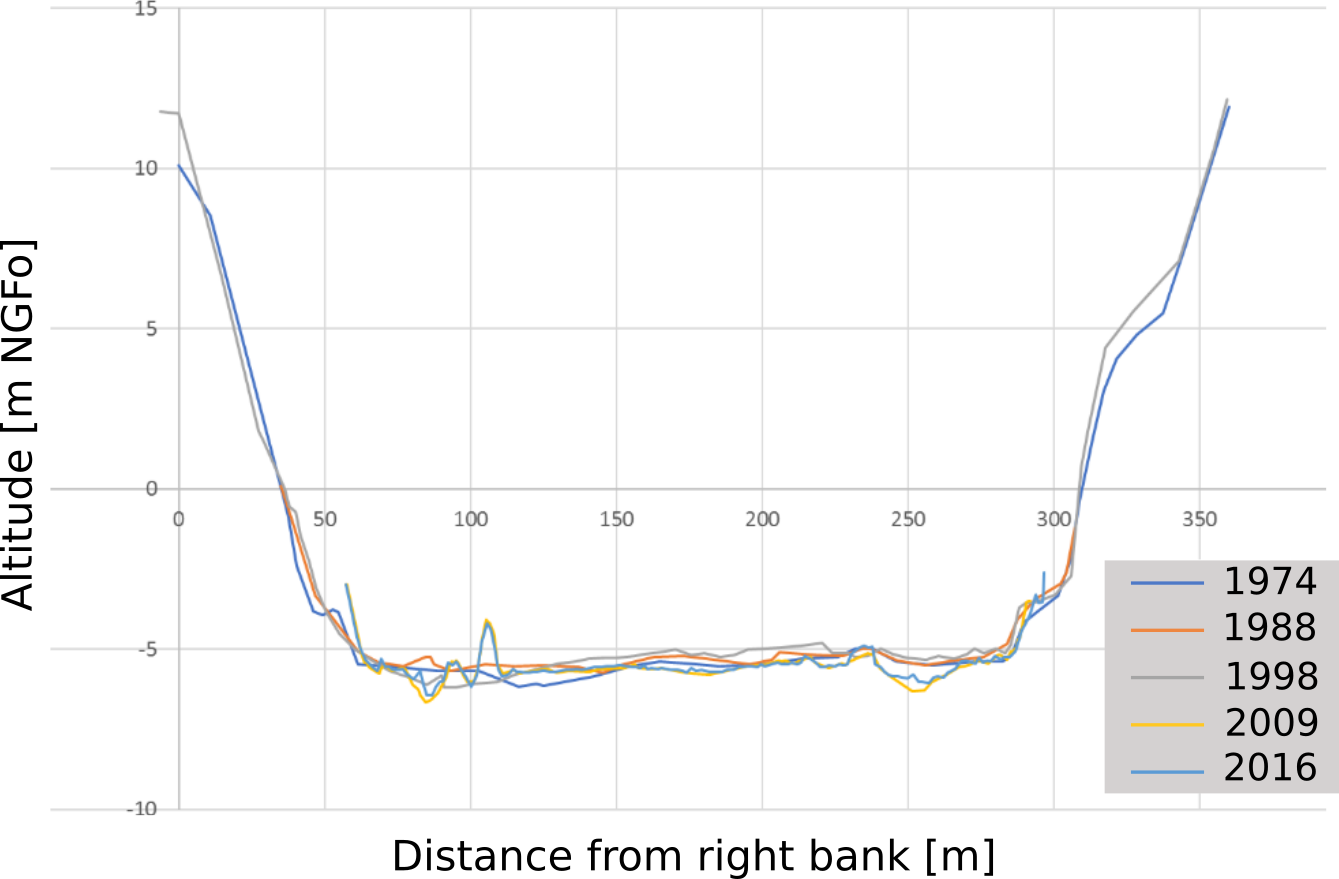
\includegraphics[width=.7\linewidth]{Figures/ProfilsBardRestit.png}
        \caption{Profils en travers du Rhône à la station de Beaucaire restitution réalisés par la CNR entre 1974 et 2016. Adapté de \cite{bard_actualisation_2018}.}	
		\label{fig:ProfilsRestit}
	\end{figure}
	
       
\FloatBarrier


\section{Données historiques : la base de données HISTRHÔNE (1300-2000)}

	\subsection{Présentation de la base de données}

	\paragraph{} La base de données HISTRHÔNE (histrhone.cerege.fr) \citep{pichard_sept_2014} regroupe près de 1500 événements hydro-climatiques, depuis le XIII\textsuperscript{ème} siècle jusqu'à la fin du XXI\textsuperscript{ème} siècle. Cet important travail d'archives qui s'est étalé sur plusieurs décennies représente un apport majeur pour la connaissance de l'histoire climatique de la basse vallée du Rhône. La zone couverte par la base de données s'étale de la ville de Pont Saint-Esprit jusqu'à la mer Méditerranée, en incluant les villes d'Avignon, Beaucaire et Arles, ainsi que l'ensemble de la Camargue (figure \ref{fig:MapHistrhone}). 
	
	\begin{figure}[h]
	\centering
		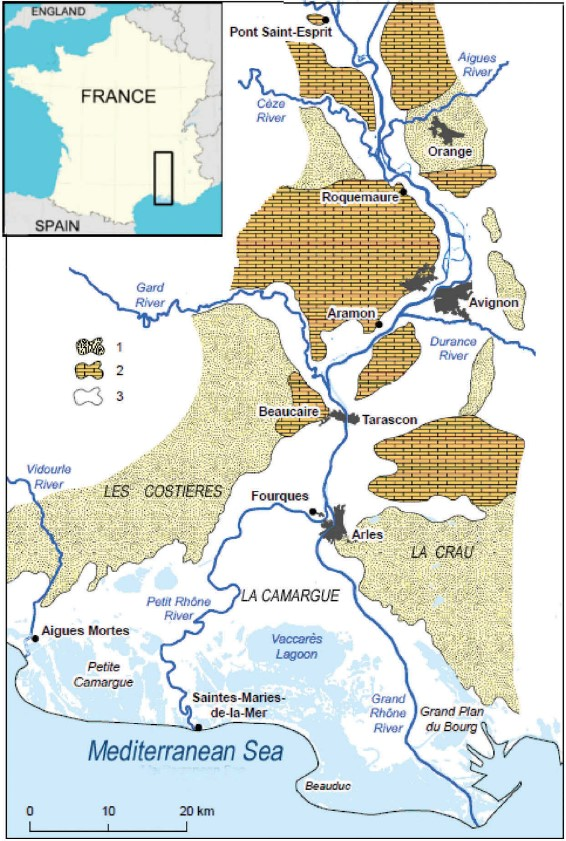
\includegraphics[width=.5\linewidth]{Figures/HistrhoneMap.jpg}
        \caption{Localisation de la zone géographique couverte par la base HISTRHÔNE \citep{pichard_sept_2014} }
		\label{fig:MapHistrhone}
	\end{figure}
	
	\paragraph{} Les éléments historiques (témoignages, cartes...) correspondant à un même événement hydroclimatique sont regroupés dans la base, et les événements sont classés par type : crue, étiage, présence de glace et gel du Rhône, inondation pluviale, submersion marine... Au delà de la base de données, l'ouvrage "Sept siècles d'histoire hydroclimatique du Rhône d'Orange à la mer" \cite{pichard_sept_2014} "offre une vue synoptique, à la fois des sources, de leur critique et des perspectives ouvertes par les premiers résultats que les auteurs ont pu en tirer comme contribution à une histoire hydroclimatique". Il faut ajouter qu'une chronologie générale des événements ainsi qu'une étude détaillée des échelles limnimétriques du bas Rhône \citep{pichard_hauteurs_2013} "reprend l'ensemble des problèmes de mesures de hauteurs des crues dans l'histoire et tente de résoudre ces complications pratiques de métrologie".
	

\FloatBarrier 
	\subsection{Catégorisation des événements de crue}
	
	\paragraph{} Dans la base de données HISTRHÔNE, les événements de crues sont classés en 6 catégories selon les dommages causés. Le tableau \ref{tab:CatCrueHistrhone} présente ces catégories
	
\begin{table}[h]
	\centering
	\caption{Classification des événements de crues de la base HISTRHÔNE. Les estimations de débit proviennent de \cite{pichard_hydro-climatology_2017}.}
	\label{tab:CatCrueHistrhone}
	\resizebox{\columnwidth}{!}{
		\begin{tabular}{|m{3cm}|m{4cm}|m{7cm}|m{3cm}|}
		\hline
		Code &
		  Libellé &
		  Description &
		  Débit estimé \\ \hline
		Ci &
		  Crue de gravité indéterminée &
		  Crue sans aucune précision : pas d'indice de débordement ni de gravité (incertitude totale) &
		  9000 \\ \hline
		Cd &
		  Crue avec indice de débordement &
		  Débordement avéré mais sans précision relative à son étendue ou sa gravité (incertitude partielle) &
		  7200 \\ \hline
		C1 &
		  Hautes eaux &
		  Rhône "pleins bords", "gros Rhône" sans débordement. Le Rhône reste dans son lit mineur mais implique une surveillance constante aux digues &
		  5200 \\ \hline
		C2 &
		  Crue avec débordement sans gravité et/ou localisé &
		  Débordement limité, sans gravité majeur ou bien localisé (ségonnaux, prés/chemins inondés, eaux sur les quais, dégâts mineurs sur digues) &
		  X \\ \hline
		C3 &
		  Crues et inondation de gravité intermédiaire &
		  Inondation notable avec dégâts avérés au caractère destructeur et/ou extension de crue &
		  X \\ \hline
		C4 &
		  Crue et inondation extrême &
		  Inondation extraordinaire avec dégâts exceptionnels (pertes humaines et animales, intérieurs des villes inondés, dégradations de digues en grand nombre) et extension de crue &
		  X \\ \hline
		\end{tabular}
	}
\end{table}
	
\FloatBarrier
	\subsection{Définition des seuils de perception}
	
	\subsection{Évolution temporelle de la perception des crues}

\section{Modélisation hydraulique des événements historiques}

	\subsection{Le modèle hydraulique MAGE}
	
	\subsection{Données disponibles utiles à la modélisaition}
	doc crues modélisables
	
	\subsection{Tests de sensibilité pour la crue de Décembre 2003}
		\subsubsection{Influence du choix des limites aval}
		
		\subsubsection{Influence des brèches}
	
	\subsection{Limites de la modélisation hydraulique des événements historiques}

\section{Évolution du temps de propagation des crues}

\section{Conclusion}

\section{Annexe : Crues modélisables}



\printbibliography
\end{document}